\section{Influence and diagnostic plots}\label{sec:logist-infl}

In ordinary least squares (OLS) regression, measures of \glossterm{influence}
(leverage, Cook's D, DFBETAs, etc.) help you to determine whether
individual cases (or cells in grouped data)
have undue impact on the fitted regression model and
the coefficients of individual predictors.
Analogs of most of these
measures have been suggested for logistic regression.
\citet{Pregibon:81} provided the theoretical basis for these methods,
exploiting the relationship between logistic models and
weighted least squares.  Some
additional problems occur in practical applications to
logistic regression because the response
is discrete, and because the leave-one-out diagnostics are more
difficult to compute.

\subsection{Residuals and leverage}
\ix{logistic regression!residuals|(}
As in ordinary least squares regression, the influence (actual impact)
of an observation in logistic models depends multiplicatively
on its residual (disagreement between $y_i$ and $\hat{y}_i$)
and its leverage (how unusual $\vec{x}_i$ is in the space of the
explanatory variables).
The multiplicative definitions imply that a case is influential to
the extent that it is poorly fit \emph{and} has unusual values of
the predictors.

In logistic regression, the simple raw residual is just $e_i \equiv y_i - \hat{p}_i$,
where $ \hat{p}_i = \exp( \vec{x}_i\trans \vec{b} ) / [1 + \exp( \vec{x}_i\trans \vec{b} )]$.
The  Pearson and deviance residuals are more useful for identifying
poorly fitted observations, and are components of overall goodness-of-fit
statistics.
The \boldital{Pearson residual} is defined as
\begin{equation}\label{eq:reschi}
r_i \equiv \frac{e_i}{\sqrt{ p_i  (1-p_i)}}
\end{equation}
and the Pearson chi-square is therefore $\chisq = \sum r_i^2$.
The \boldital{deviance residual} is
\begin{equation}\label{eq:resdev}
g_i \equiv \pm { -2 [ y_i \log p_i  + (1-y_i) \log (1-p_i) ] }^{1/2}
\end{equation}
where the sign of $g_i$ is the same as that of $e_i$.
Likewise, the sum of squares of the deviance residuals gives
the overall deviance,
$G^2 = -2 \log \mathcal{L}(\vec{b}) = \sum g_i^2$.

When $y_i$ is a binomial count based on $n_i$ trials (grouped data),
the Pearson residuals \eqref{eq:reschi} then become
\begin{equation*}%\label{eq:reschi2}
r_i \equiv \frac{y_i -n_i p_i}{\sqrt{n_i  p_i  (1-p_i)}}
\end{equation*}
with similar modifications made to \eqref{eq:resdev}.
\ix{logistic regression!residuals|)}

\ix{logistic regression!leverage|(}
Leverage measures the \emph{potential} impact of an individual case
on the results, which is directly proportional to how far an
individual case is from the centroid in the space of the
predictors.  Leverage is computed as the diagonal elements,
\(h_{ii}\), of the ``Hat'' matrix, \(\mat{H}\),

\begin{equation*}%\label{eq:}
\mat{H} = {\mat{X}}^\star
{( {\mat{X}^\star}\trans {\mat{X}}^\star )}^{-1} {\mat{X}^\star}\trans
\end{equation*}
where \({\mat{X}} ^\star = {\mat{V}}^{1/2} \mat{X}\), and \(\mat{V}  =
\diag [ \hat{\vec{p}} ( 1 - \hat{\vec{p}})] \).  As in OLS,
leverage values are between 0 and 1, and a leverage value,
\(h_{ii}  > 2 (k+1) /  n\) is considered ``large''; here, \(k\) is the
number of predictors, and \(n\) is the number of cases.
In OLS, however, the hat values depend only on the $X$s, whereas
in logistic regression, they also depend on the dependent
variable values and the fitted probabilities (through $\mat{V}$).
As a result, an observation may be extremely unusual on the predictors,
yet not have a large hat value, if the fitted probability is near 0 or 1.
\ix{logistic regression!leverage|)}

\subsection{Influence diagnostics}\label{sec:logist-infldiag}
\ix{logistic regression!influence diagnostics|(}
Influence measures assess the effect that deleting an
observation has on the regression parameters, fitted values, or the
goodness-of-fit statistics.  In OLS, these measures
can be computed exactly from a single regression.
In logistic regression, the exact effect of deletion
requires refitting the model with each observation deleted in turn
(because the estimating equations \eqref{eq:like4} are nonlinear),
a time-intensive computation.
Consequently, \citet{Pregibon:81} showed how analogous deletion
diagnostics may be approximated by performing one additional step
of the iterative procedure.

The simplest measure of influence of observation $i$ is the standardized change in the coefficient for each variable due to omitting that observation,
termed \boldital{DFBETA}s.  From the relation \citep[p. 716]{Pregibon:81}
\begin{equation*}%\label{eq:dfbetas}
 \vec{b} -  \vec{b}_{(-i)} = (\mat{X}\trans \mat{V} \mat{X})^{-1} \vec{x}_i (y_i - p_i) / (1 - h_{ii})
 \comma
\end{equation*}
the estimated standardized change in the coefficient for variable $j$ is
\begin{equation}\label{eq:dfbeta}
 \mbox{DFBETA}i_j \equiv \frac{b_{(-i)j} -  b_j } {\hat{\sigma} (b_j)}
 \comma
\end{equation}
where $\hat{\sigma} (b_j)$ is the estimated standard error of $b_j$.
With $k$ regressors, there are $k+1$ sets of DFBETAs, which makes their examination burdensome.
Graphical displays ease this burden, as do various summary measures
considered below.

The overall influence of observation $i$ on the estimated regression
coefficients is assessed by analogs of \glossterm{Cook's distance}, which measure
the difference between $\vec{b}$ for all the data and
$\vec{b}_{(-i)}$ estimated without observation $i$.
One measure, $C_i$, is defined as
\begin{equation*}%\label{eq:cookd1}
C_i \equiv ( \vec{b} - \vec{b}_{(-i)} )\trans \:
    \mat{X}\trans \mat{V} \mat{X} \:
     ( \vec{b} - \vec{b}_{(-i)} )
	  \comma
\end{equation*}
and calculated as
\begin{equation}\label{eq:cookd2}
 C_i = \frac{r_i^2 h_{ii}} {(1-h_{ii} )^2}
 \period
\end{equation}
A second measure, $\overline{C}_i$, is calculated as
\begin{equation}\label{eq:cookd3}
 \overline{C}_i = \frac{r_i^2 h_{ii}} {(1-h_{ii} )} = (1-h_{ii} ) C_i
 \period
\end{equation}
Because $0 \le h_{ii} \le 1$, $\overline{C}_i$ will never be larger than $C_i$.
These measures are referred to by the keywords \pname{C} and
\pname{CBAR}, respectively, on the \stmt{OUTPUT}{LOGISTIC}.
Both can be interpreted as squared measures of the change in
size of the confidence intervals for all regression coefficients.
Rules of thumb for noticeably large values are necessarily only
rough indicators, but \citet{Johnson:85} suggests comparing $k C_i$
to a $\chi^2 (k)$ distribution.

The Pearson and deviance residuals defined above do not have equal
variance, but rather have variance $\approx 1-h_{ii}$.  Studentized versions
of both which do have equal variance
are obtained by dividing by $\sqrt{1-h_{ii}}$.  For example, the
studentized deviance residual (\pname{RESDEV}) is $g_i^\star = g_i /
\sqrt{1-h_{ii}}$.
These are most usefully expressed in squared form as the approximate decrease in the
deviance (\pname{DIFDEV}) and Pearson (\pname{DIFCHISQ}) \chisq\ 
associated with deleting observation $i$:
\begin{equation*}%\label{eq:difdev}
  \Delta G_{(-i)}^2 = \frac{g_i^2}{1-h_{ii}}
  \comma
\end{equation*}
and
\begin{equation*}%\label{eq:chi}
  \Delta \chi_{(-i)}^2 = \frac{r_i^2}{1-h_{ii}}
  \period
\end{equation*}
These are both asymptotically distributed as $\chi^2 (1)$, so a value
exceeding 3.84 (or the rounded value, 4) is worth noticing.
They may also be interpreted as indicating how poorly the current
model fits observation $i$.

As with OLS, influential observations signal something unusual:
extreme (or erroneous) predictor values combined with an ill-predicted
response, e.g., someone who died, but should have survived (according to the
model).  They may also signal that some important (perhaps unmeasured)
predictor--- a lurking variable--- has been omitted from the model \citep{Joiner:81} or expressed
on the wrong scale.

\subsection{Influence output from \PROC{LOGISTIC}}
All the influence statistics are
printed when the \opt{influence}{LOGISTIC} is used on the \stmt{MODEL}{LOGISTIC}.
For example, we get these diagnostics for the arthritis data with:
\begin{listing}
proc logistic data=arthrit ;
   model better = _sex_ _treat_ _age_ / influence;
\end{listing}

This produces many pages of output, of the form in \outref{out:glogist3.1},
shown for two of the many diagnostic measures.
With so much output, it is often difficult
to spot unusual observations.  A more useful option, \pname{IPLOTS},
produces index plots of each of the diagnostic measures against
the observation index, with the goal of showing which observations
stand out from the rest.
It is even more useful, I believe, to plot certain diagnostics
against each other, including reference lines showing the nominal
danger-level for each diagnostic,  because they help to pinpoint
\emph{why} certain observations are influential.
Some examples of these plots are described in the following subsection.

\begin{Output}[htbp]
\caption{Regression diagnostics, printed output (partial) for arthritis data}\label{out:glogist3.1}
\small
\verbatiminput{ch6/out/glogist3.1}
\end{Output}

\subsection{Diagnostic plots of influence measures}
Plots of the change in \(\chi^2\) (\pname{DIFCHISQ} or \pname{DIFDEV}) against
either leverage or predicted probability are particularly useful
for detecting unduly influential cases.
These are discrete analogs of plots recommended for linear models
by \citet{Fox:91} and \citet{Friendly:91}.
The estimated overall
influence of each case on the estimated coefficients ($C_i$ or $\overline{C}_i$)
can be shown in a bubble plot where the plotting symbols are circles
proportional to \pname{C} or \pname{CBAR}.

Such plots are produced by the \macro{INFLOGIS},
described in \macref{mac:inflogis}.  For example, these
statements produce plots of DIFCHISQ against both the 
predicted probability, \pname{PRED} 
(\figref{fig:logi1b1}) and
leverage, \pname{HAT}
(\figref{fig:logi1b2}),
using bubbles whose area is proportional
to C:
%% \input{logist1b} %% level: 2
\begin{listing}
title 'Arthritis treatment data';
title2 'Bubble size: Influence on Coefficients (C)';
goptions htext=1.6;
%include data(arthrit);
%inflogis(data=arthrit,
     y=better,               /* response   */
     x=_sex_ _treat_ age,    /* predictors */
     id=id,                  /* case label */
     gy=DIFCHISQ,            /* graph ordinate  */
     gx=PRED HAT,            /* graph abscissas */
     lcolor=RED, bsize=14
     );
\end{listing}

The printed output from the \macro{INFLOGIS} includes a table
identifying any observation of high leverage \emph{or} high influence.
These observations are also labeled in the graphs.  For
example, case 29 is of high leverage, because she is unusual in terms
of the predictors: a young woman given treatment; however, she is not
influential in the fitted model.  Case 77, is not of high leverage,
but is poorly predicted by the model and has a large contribution to
\chisq.

\begin{output}
CASE BETTER  _SEX_  _TREAT_  AGE   HAT  DIFCHISQ   DIFDEV     C

  1     1      0       1      27   .09    4.5781   3.6953   0.4510
 22     1      0       0      63   .06    4.4603   3.5649   0.2898
 29     0      1       1      23   .14    1.0183   1.4005   0.1679
 30     1      1       0      31   .05    4.7485   3.6573   0.2611
 34     1      1       0      33   .05    4.2955   3.4644   0.2236
 55     0      1       1      58   .03    4.9697   3.6759   0.1602
 77     0      1       1      69   .03    8.4977   4.7122   0.2758
\end{output}

\begin{figure}[!htb]
  \centering
  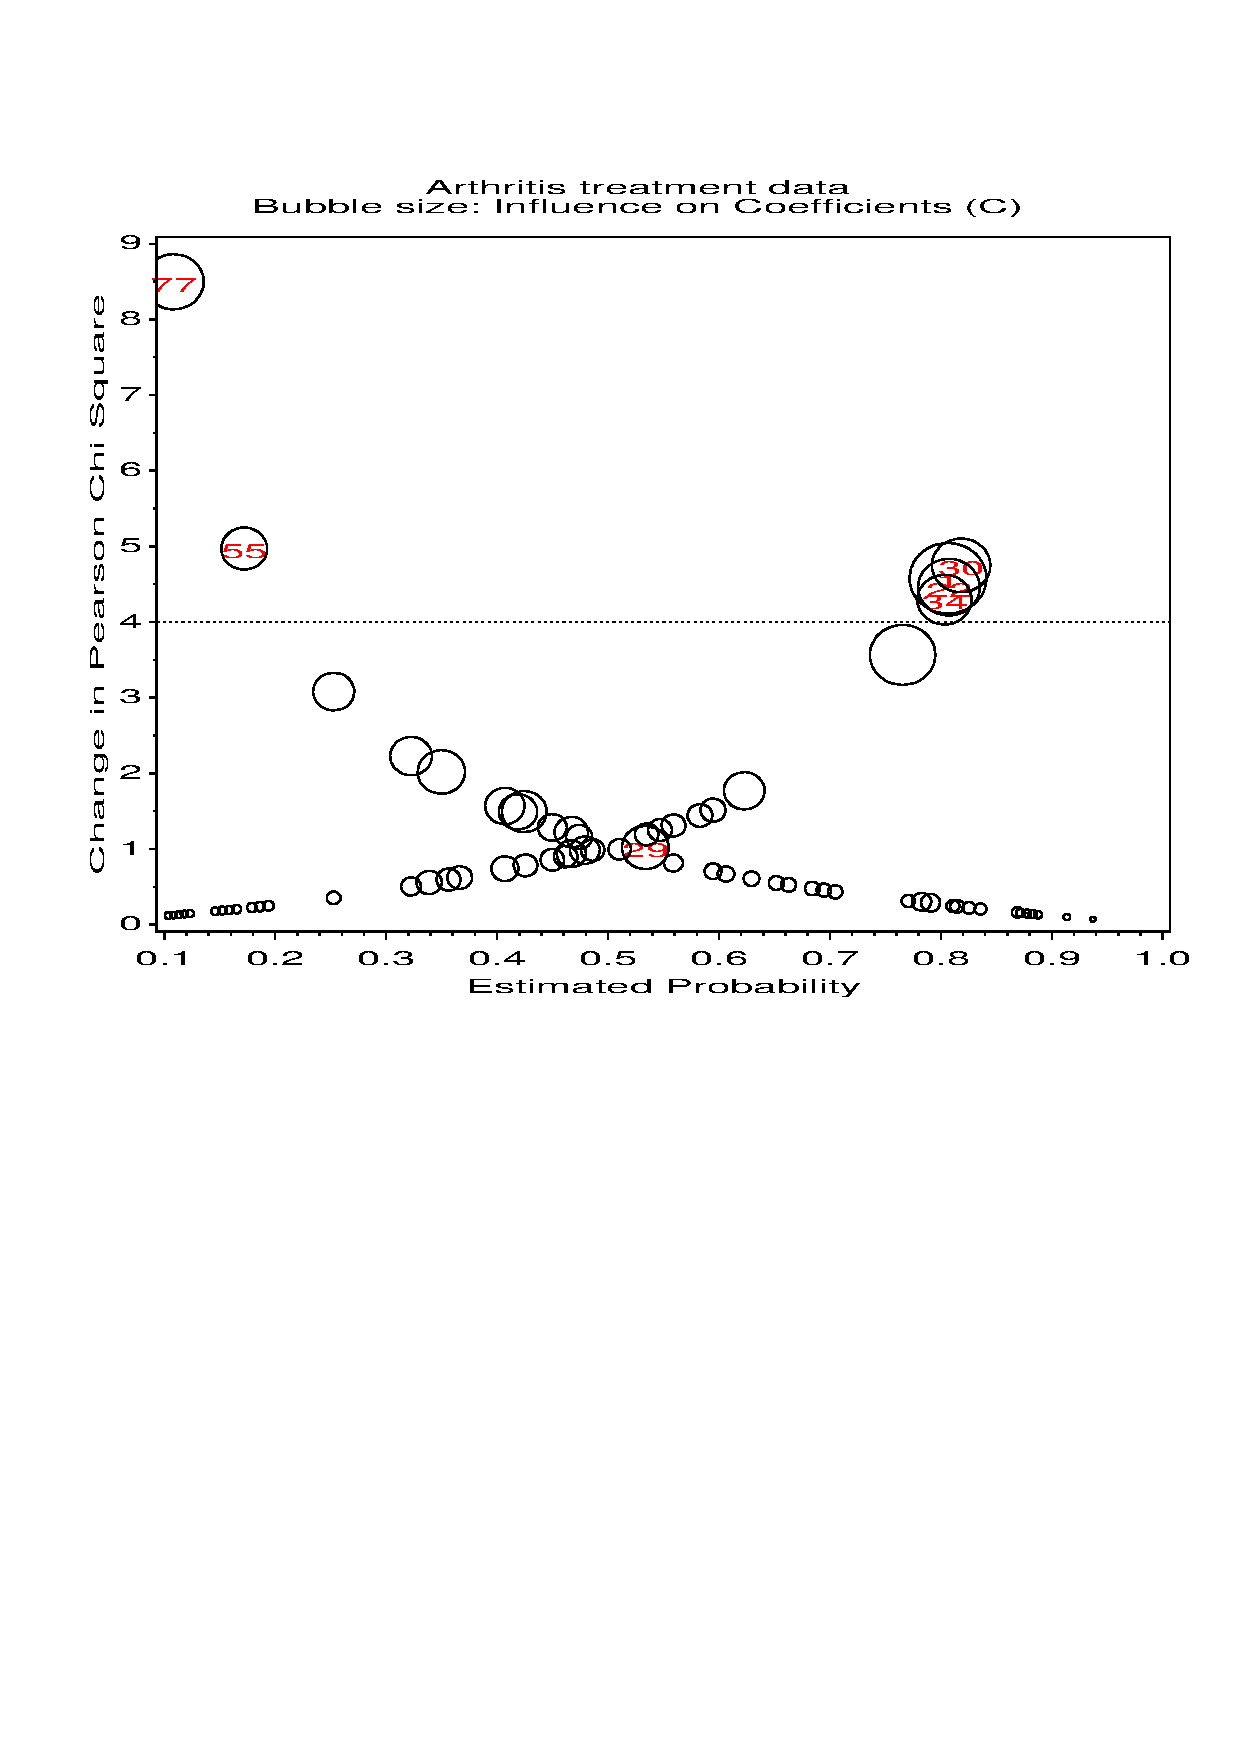
\includegraphics[scale=.7]{ch6/fig/logist1b1}
  \caption[Influence plot for arthritis data]{Influence plot for arthritis data.
Cases with DIFCHISQ \(> 4\) or leverage \(>  (2 k) /  n  = 0.095\) are
labeled as
influential, as indicated by the size of the bubble symbol.
The systematic pattern shown is inherent in the discrete nature of
logistic regression.  The most influential
observations are those with very high or low predicted probabilities.}\label{fig:logi1b1}
\end{figure}

\begin{figure}[!htb]
  \centering
  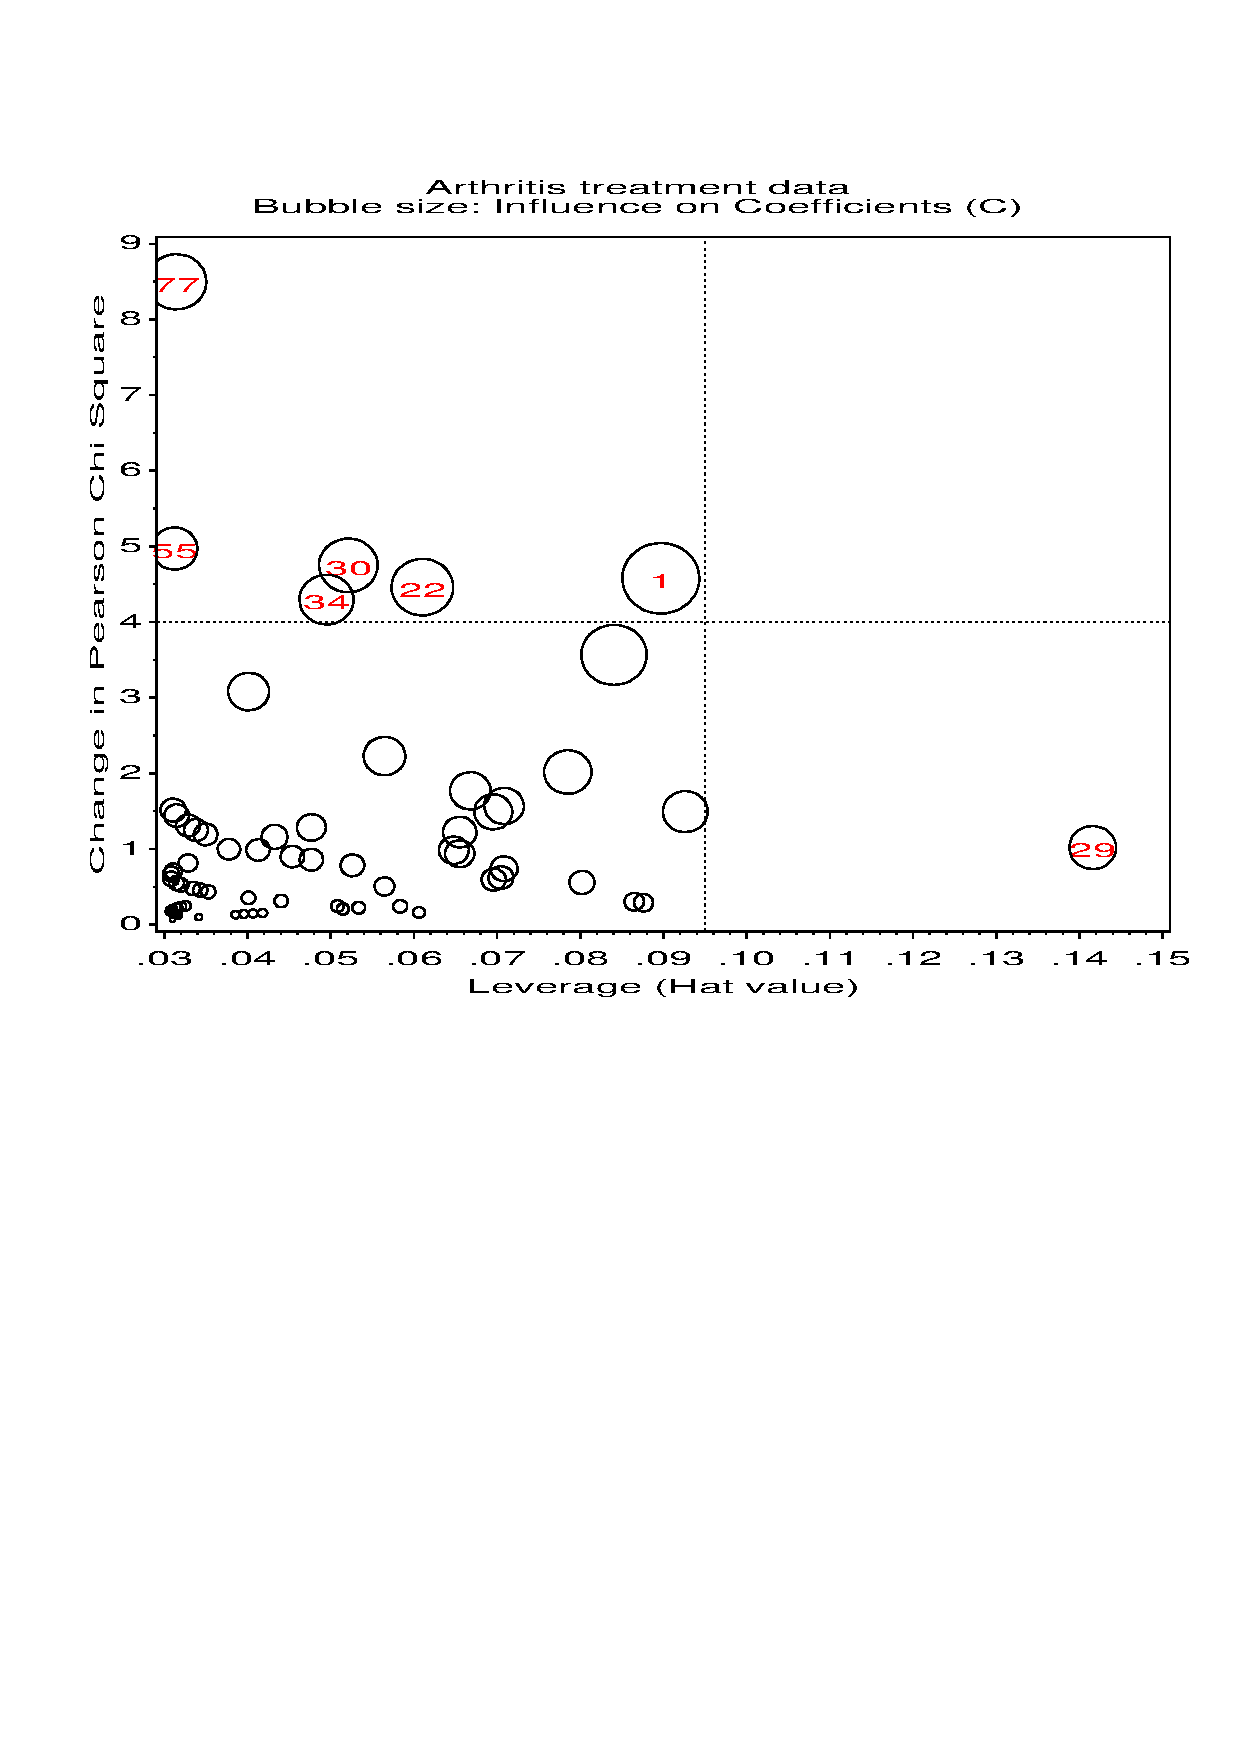
\includegraphics[scale=.7]{ch6/fig/logist1b2}
  \caption[Changes in chi-square vs. leverage]{Changes in chi-square vs.\ leverage.
  The same cases are labeled as in \figref{fig:logi1b1}.
}\label{fig:logi1b2}
\end{figure}
\ix{logistic regression!influence diagnostics|)}

\begin{Example}[icu2]{Survival in the ICU}
The four variable model from \exref{ex:icu1} predicting survival in the ICU
was examined for influential cases with the \macro{INFLOGIS}.
The following macro call produces an influence plot of the \pname{DIFCHISQ}
statistic against hat values, shown in \figref{fig:icu12}.
\begin{listing}
%inflogis(data=icu, y=died, x=age cancer uncons admit,
   id=id,
   gy=difchisq,
   gx=hat);
\end{listing}

%% one figure
\begin{figure}[htb]
  \centering
  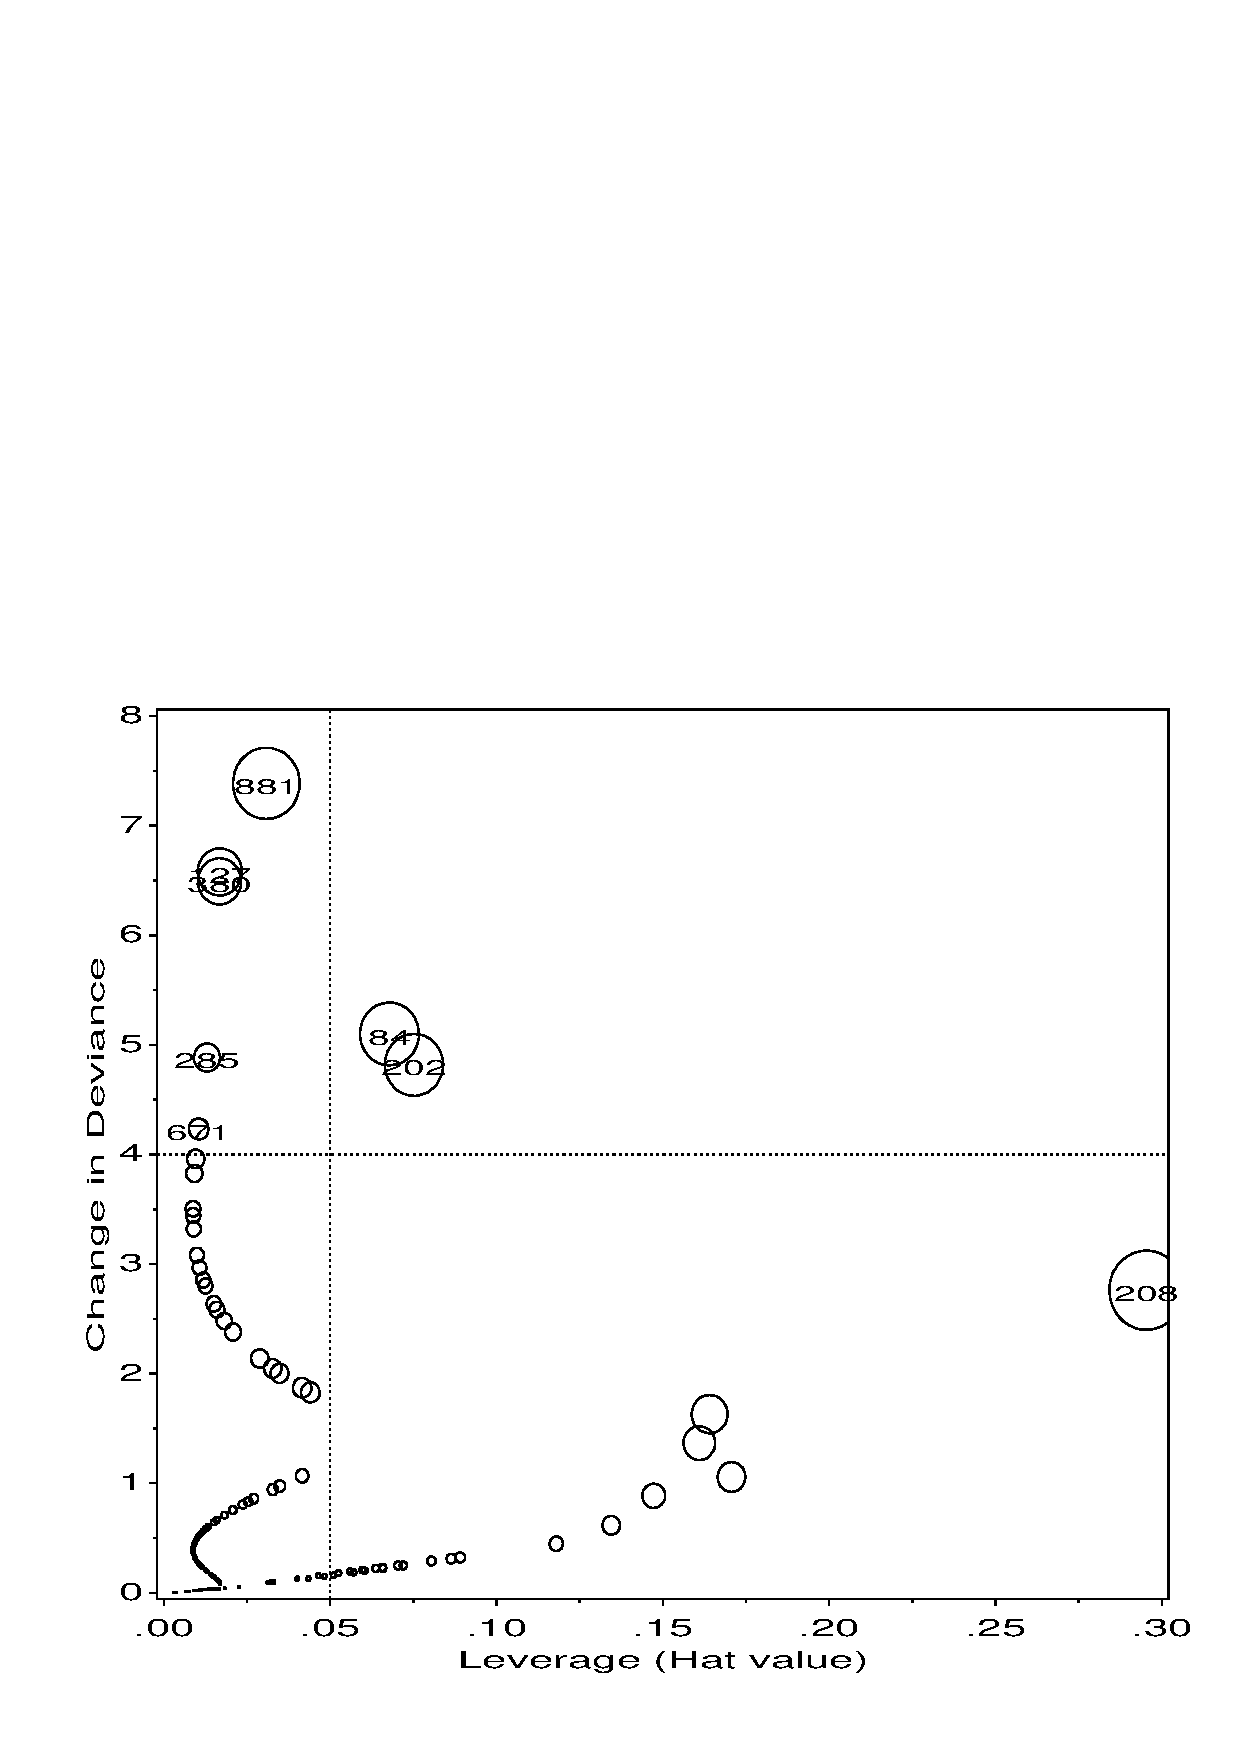
\includegraphics[scale=.6]{ch6/fig/icu12}
  \caption[ICU Survival data: Influence plot]{ICU Survival data: Influence plot}%
  \label{fig:icu12}
\end{figure}

Details for the cases identified in the figure are shown in \outref{out:icu1.2}.
None of the cases are particularly influential on the model coefficients overall:
the largest $C_i$ is only 1.04.
Case 208, with the largest hat value, is unusual on the predictors
in this sample: a 70 year old man without cancer, admitted on an elective
basis (who nonetheless died).
On the other hand, case 881, an 89 year old male, admitted unconscious
as an emergency case is poorly predicted because he survived.
Similarly, two other cases (127, 380) with large $\Delta \chi_{(-i)}^2$
are poorly predicted because they died, although they were
young, did not have cancer, and conscious at admission.
From this evidence we might conclude that none of these cases greatly affects the model, its coefficients,
or interpretation.
\begin{Output}[htb]
\caption{ICU data: Influential cases}\label{out:icu1.2}
\small
\verbatiminput{ch6/out/icu1.2}
\end{Output}

That conclusion might not be warranted without further study, particularly
in terms of influence on individual coefficients.
The DFBETAs \eqref{eq:dfbeta} may be obtained in an \ODS\ as shown below:
\begin{listing}
proc logistic data=icu;
   model died = age admit cancer uncons;
   output out=stats dfbetas=dbint dbage dbadmit dbcancer dbuncons ;
\end{listing}

%% two subfig side-by-side
\begin{figure}[htb]
 \begin{minipage}[t]{.49\linewidth}
  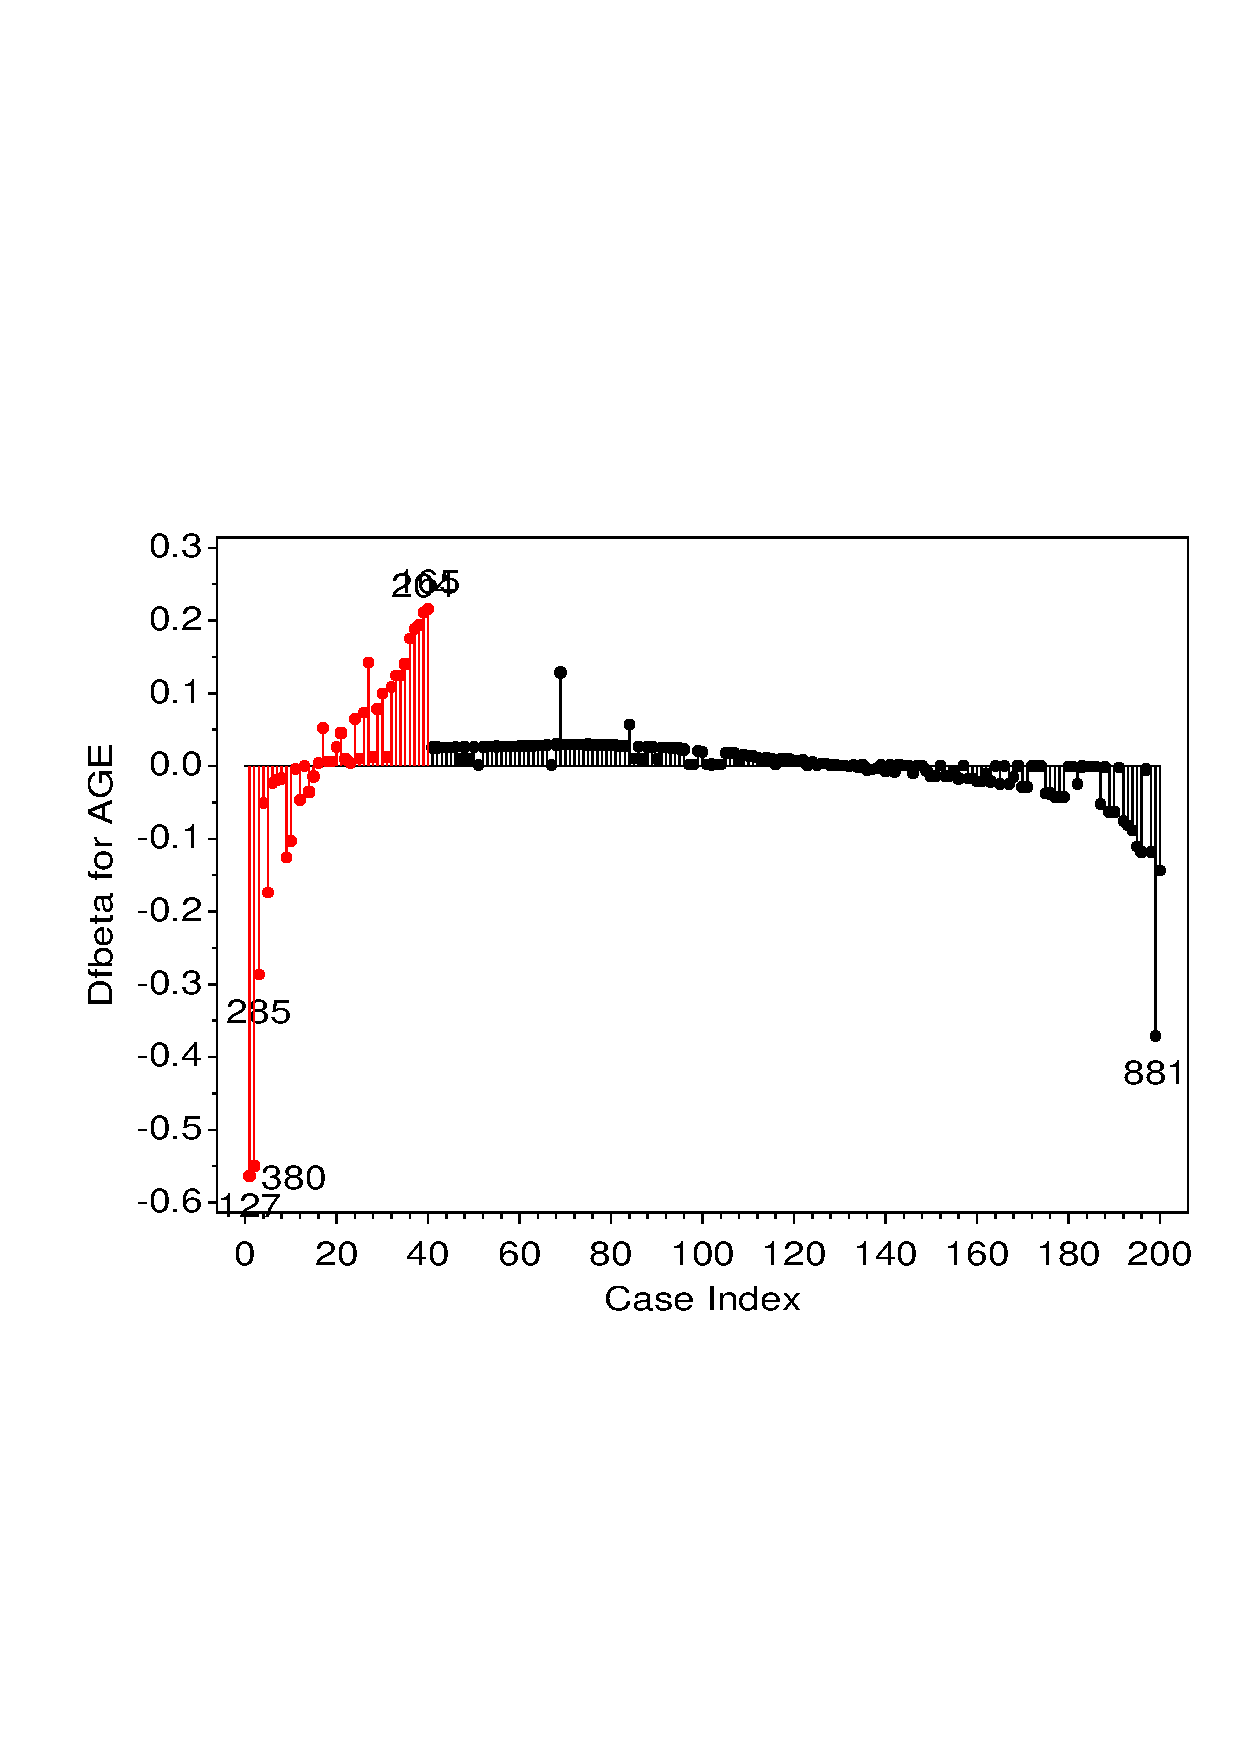
\includegraphics[width=1\linewidth,clip]{ch6/fig/icu4b1}
 \end{minipage}%
 \hfill
 \begin{minipage}[t]{.49\linewidth}
  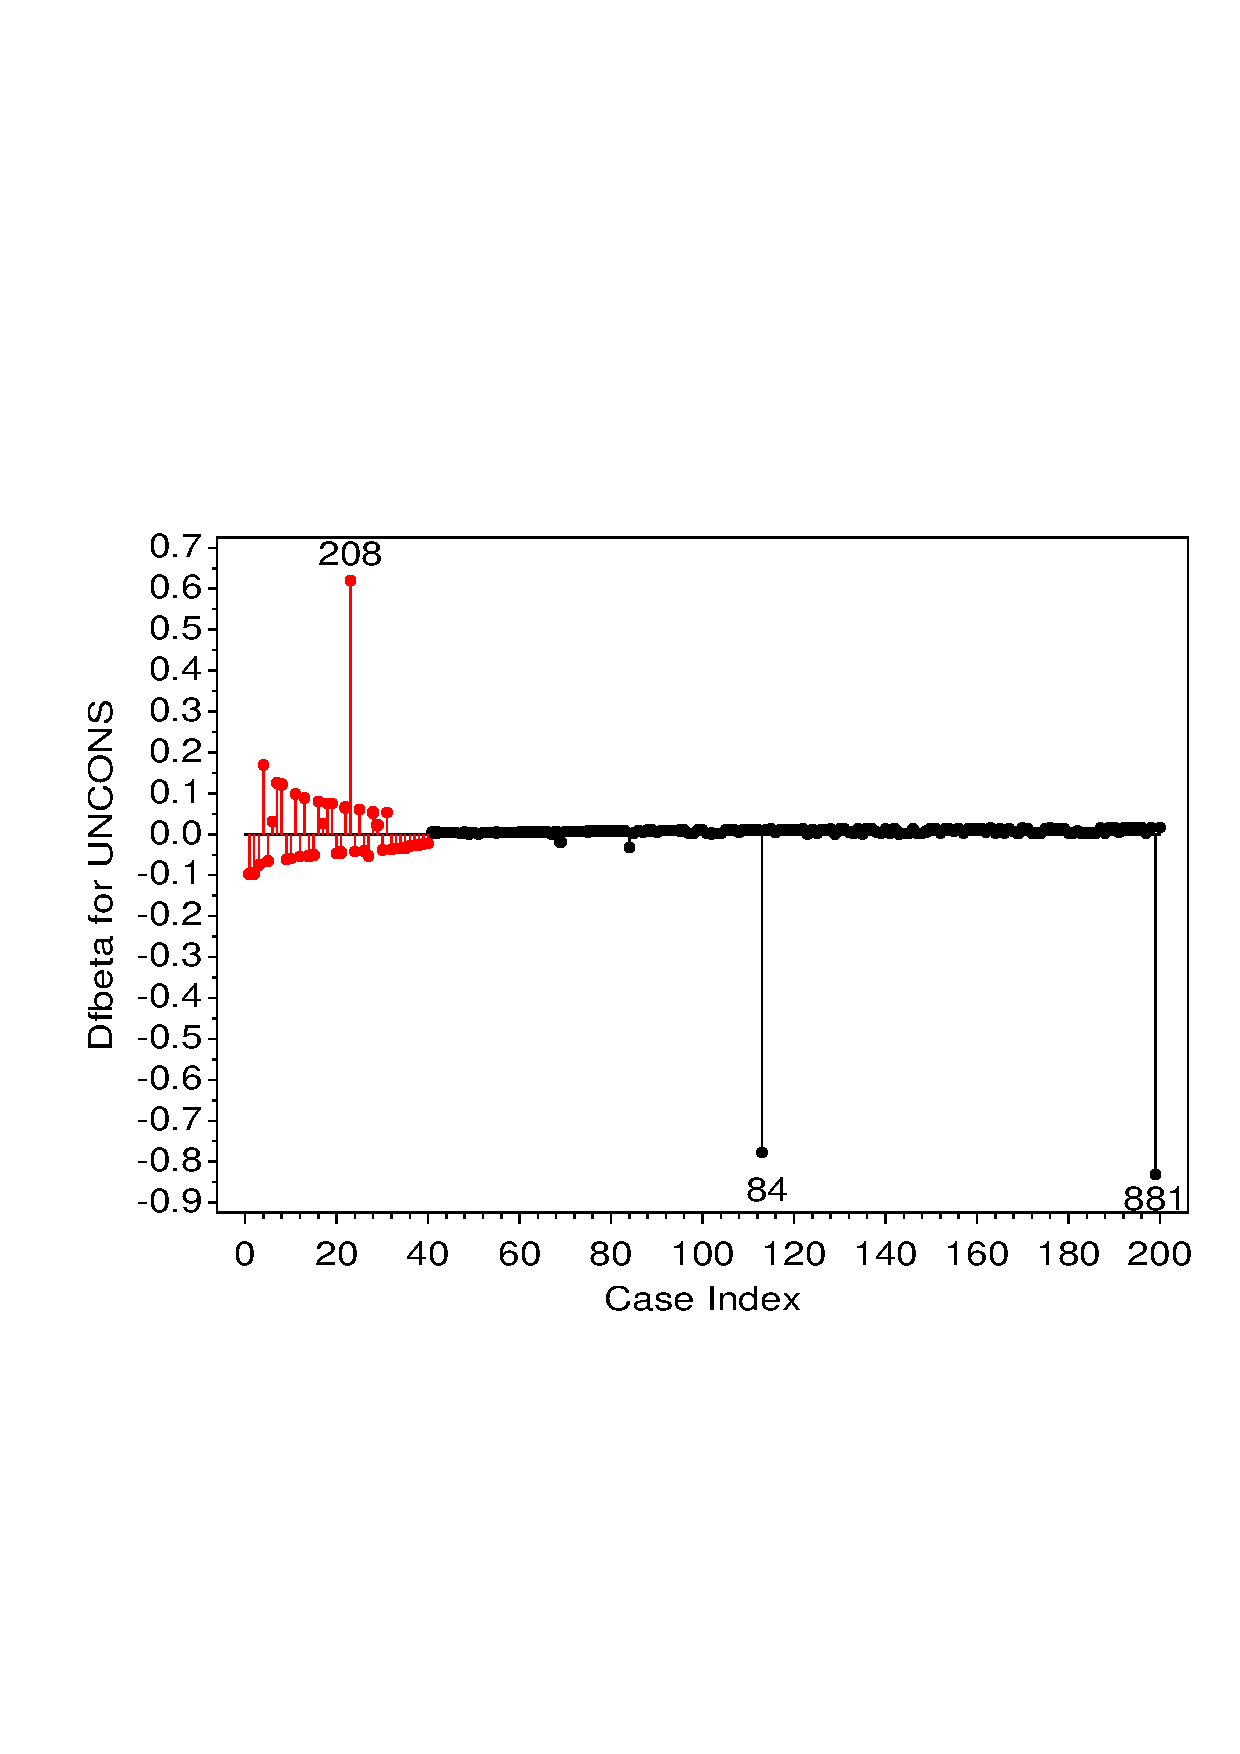
\includegraphics[width=1\linewidth,clip]{ch6/fig/icu4b2}
 \end{minipage}
 \caption{ICU data: DFBETA index plots for Age and Uncons}\label{fig:icu4b}
\end{figure}
Individual DFBETAs are often graphed as \emph{index plots}, that is,
for variable $j$ a plot of DFBETA$(i, j)$ against the case index $i$.
In such plots, it is helpful to label points with large absolute
values when (as here) the case number is not meaningful.
For example, the following statements produce an index plot of the
DFBETA for age, shown in \figref{fig:icu4b}.
The \macro{LABEL} is used to label points by the patient \pname{id},
where the DFBETA value exceeds 0.2 (an arbitrary value) in magnitude.
\begin{listing}
data stats;
   set stats;
   case = _n_;

%label(data=stats, x=case, y=dbage, text=put(id,3.), pos=-,
    subset=abs(dbage)>.2, out=labs);

proc gplot data=stats;
   plot dbage * case = died /
      anno=labs frame nolegend vaxis=axis1 haxis=axis2 vm=1;
   symbol1 i=needle v=dot c=black;
   symbol2 i=needle v=dot c=red;
   axis1 label=(a=90) length=4.5in;
   axis2 offset=(2) ;
\end{listing}
An alternative display, which is often more informative (though possibly more complex) is a scatterplot matrix of the DFBETAs, perhaps with other
influence diagnostics as well.
The pairwise scatterplots help to highlight observations which are
influential on both or only one of each pair of measures.
An example is shown in \figref{fig:icu4a}, produced with the
\macro{SCATMAT}:
\begin{listing}
%scatmat(data=stats,
   var= dbAge dbAdmit dbCancer dbUncons, group=died,
   symbols=star square,
   plotopt=%str(href=-0.2 0.2 vref=-0.2 0.2 cvref=graya0 chref=graya0));
\end{listing}

%% one figure
\begin{figure}[htb]
  \centering
  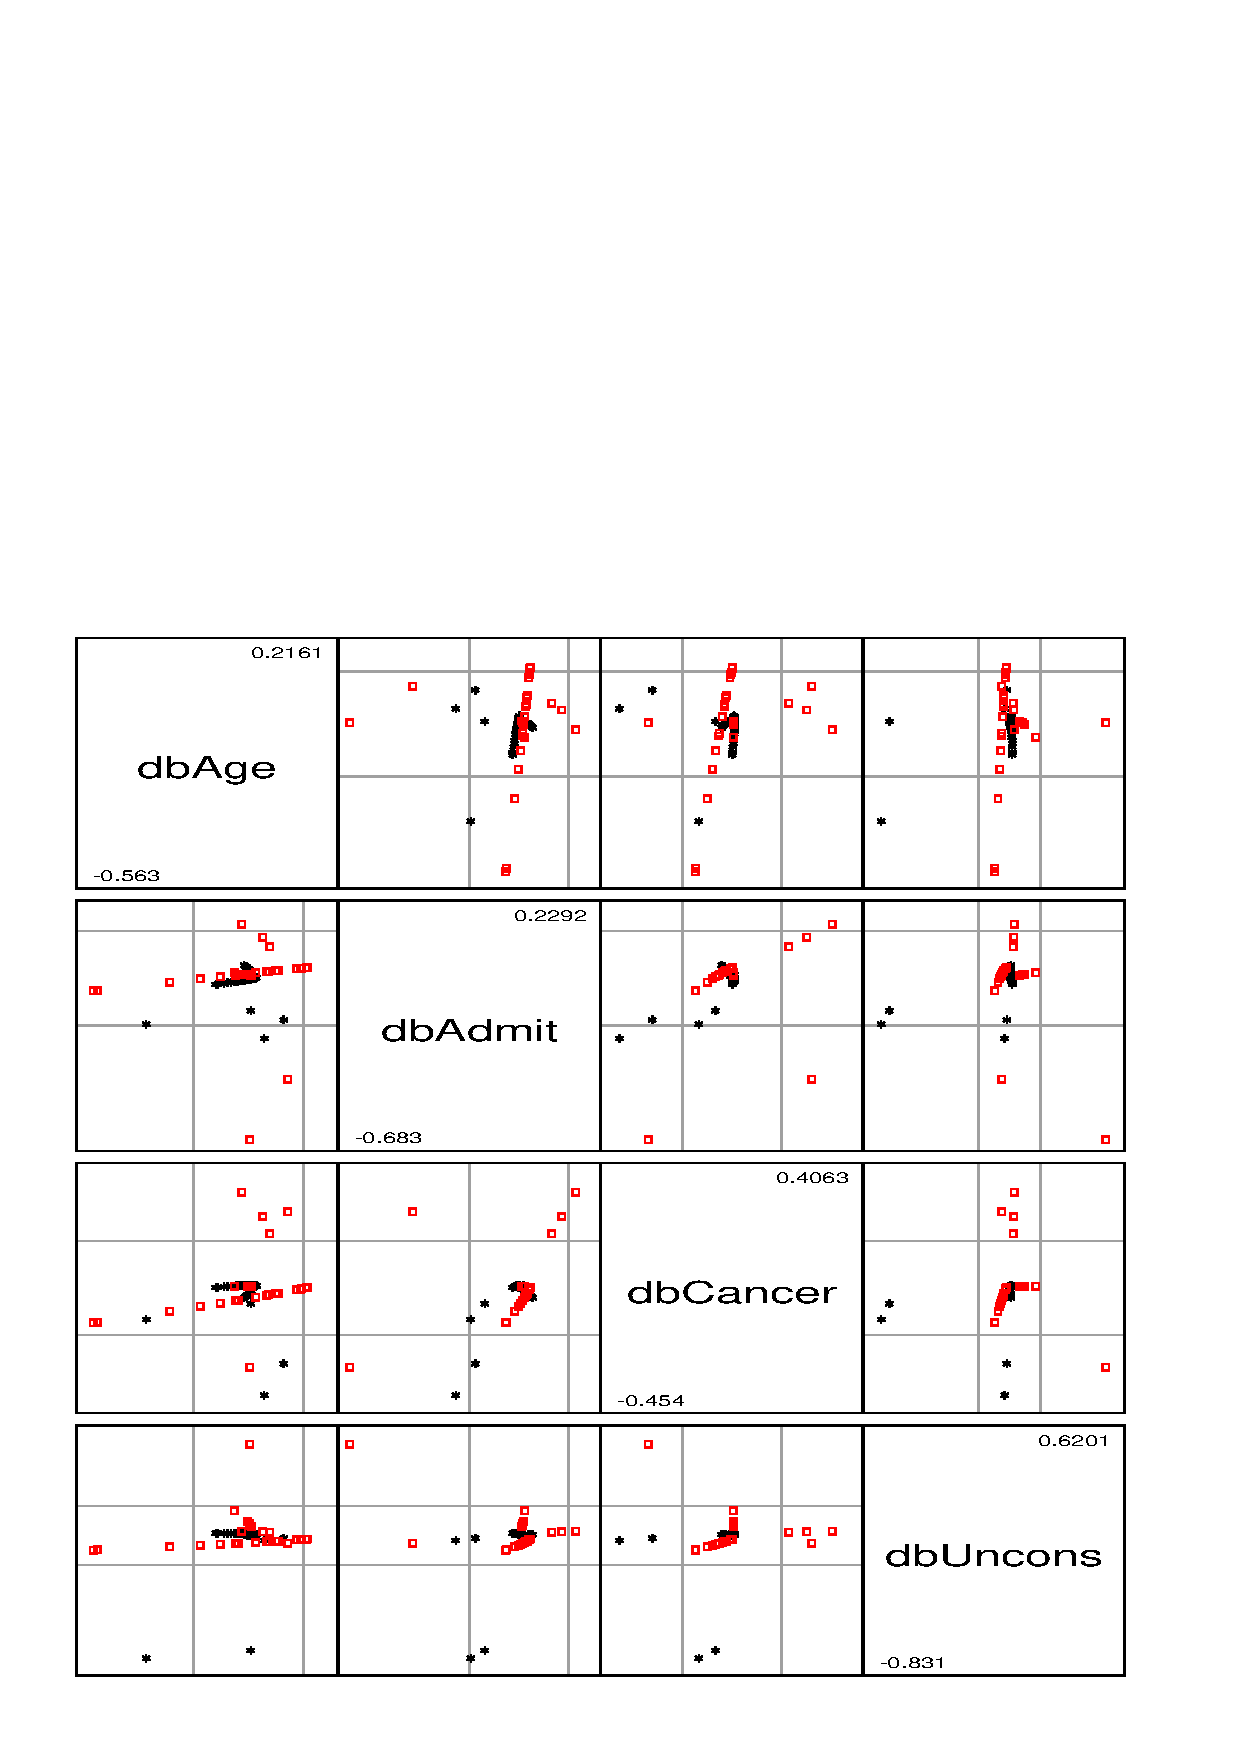
\includegraphics[scale=.75]{ch6/fig/icu4a}
  \caption[ICU Survival data: Scatterplot matrix of DFBETAs]{ICU Survival data: Scatterplot matrix of DFBETAs.  Those who lived are shown by $\star$s,  those who died are shown by squares.
  The reference lines indicate values of $\pm 0.2$ on each statistic.}%
  \label{fig:icu4a}
\end{figure}
Most of the observations are in the central rectangle, corresponding to
small values ($< \pm 0.2$) on both measures, but several points stand out
on the pairwise combinations.  For example, the bottom row and
rightmost column (DFBETA for \pname{UNCONS})
highlight two observations for patients who lived ($\star$s)
whose omission would decrease the coefficient for \pname{UNCONS}
considerably, and one who died whose omission would increase it.
Other observations outside the central rectangle might also be investigated.
\end{Example}

\subsection{Partial residual and added-variable plots}\label{sec:logist-partial}
The graphical methods described in this section are relatively
straight-forward indicators of the adequacy of a particular model,
with a specified set of predictors, each expressed in a given way.
More sophisticated methods have also been proposed, which focus on the need to include a particular predictor and whether its relationship is linear.
These include the \glossterm{partial residual plot},
\glossterm{added-variable plot}, and the
\glossterm{constructed variable plot},
which are all analogous to techniques developed in OLS.

\subsubsection{Partial residual plots}
The partial residual plot \citep{LarsenMcCleary:72} is designed to
show whether a given variable, $x_j$, included linearly in the model,
actually shows a nonlinear relation, requiring transformation.
As adapted to logistic regression by \citet{Landwehr-etal:84},
the partial residual for variable $x_j$ is defined as
\begin{equation*}%\label{eq:partres}
\vec{r}^{\star} = \mat{V}^{-1} \vec{r} + \beta_j \vec{x}_j
 = \frac{\vec{y} - \vec{p}}{ \vec{p} (1 - \vec{p})} \period
\end{equation*}
The partial residual plot is then a plot of $\vec{r}^{\star}$ against
$\vec{x}_j$, possibly with the addition of a smoothed lowess curve
\citep{Fowlkes:87} and
a linear regression line to aid interpretation.
If $x_j$ affects the binary response linearly, the plot should be approximately linear with a slope approximately equal to $\beta_j$.
A nonlinear plot suggests that $x_j$ needs to be transformed, and
the shape of the relation gives a rough guide to the required
transformation.
For example, a parabolic shape would suggest a term in $x_j^2$.

\subsubsection{Added variable plots}
The added variable plot, developed for generalized linear models by
\citet{WangP:85}, is a diagnostic plot designed to indicate whether
some new regressor, $z$, should be added to the model
which includes other explanatory variables.
An overall test could be based on the difference in $G^2$ for
the enlarged model $\logit(\vec{p}) = \mat{X} \vec{\beta} + \gamma \vec{z}$,
compared to the reduced model
$\logit(\vec{p}) = \mat{X} \vec{\beta}$.
But the added variable plot shows whether the evidence for including
$z$ is spread throughout the sample or confined to a small subset
of observations.
The regressor $z$ may be a new explanatory variable, or a higher power
of a variable already in the model.

The added variable plot may be constructed by following the logistic
regression for the reduced model with the variables in $\mat{X}$
with one weighted least squares regression of $\vec{z}$ on
$\mat{X}$ to find the residual part, $z^{\star}$,  of $z$ not predicted
by the previous regressors.
Let $\vec{r}$ be the vector of Pearson residuals from the initial logistic
fit of $\vec{y}$ on the variables in $\mat{X}$,
and let $\mat{H}$ and $\mat{V} = \diag [ \hat{\vec{p}} ( 1 - \hat{\vec{p}})]$
be the hat matrix and V matrix from this analysis.
Then, the added variable plot is a \scat\ of
the residuals $\vec{r}$ against the $z$-residuals,
\begin{equation*}%\label{eq:addvar}
 \vec{z}^{\star} = ( \mat{I} - \mat{H} ) \mat{V}^{1/2} \vec{z} \period
\end{equation*}
The $z$-residuals are easily calculated as
$z_i^{\star} = ( z_i - \hat{z}_i ) \sqrt{v_{ii}}$,
where $\hat{z}_i$ is the fitted value of $z_i$
in a weighted least squares regression of $\vec{z}$ on $\mat{X}$
using the $v_{ii}$ as weights.

A linear relation in this plot indicates that $z$ should be included in the
model, but observations with extreme $z$-residuals would be highly
influential in this decision.  A line fitted to this plot should have
an intercept approximately zero, and a slope approximating the coefficient
$\gamma$ of $z$ in the full model.
Added variable plots are produced by the \macro{ADDVAR}, described
in \macref{mac:addvar} and illustrated in the following example.

\begin{Example}[icu3]{Survival in the ICU}
In \exref{ex:icu1} we saw that the backward selection method nominated
three other variables, Systolic, pH, and PCO in addition to the four
variables we have been using throughout.
Here we first investigate whether systolic (blood pressure) should be
added to the model which includes Age, Admit, Cancer and Uncons.

The \macro{ADDVAR} is called as follows, to produce \figref{fig:icu61}.
There is no evidence of a strong linear relation, suggesting that
Systolic blood pressure has only a weak relationship to the residual in the current model.  The smooth lowess curve suggests
that any relationship may
be mildly quadratic
(though partial residual plots are generally preferable for detecting
nonlinearity).
The labeled points are those whose studentized Pearson residuals
exceed 2 in absolute value.
\begin{listing}
%addvar(data=icu,
   y=Died,                       /* response */
   x=age admit cancer uncons,    /* original predictors */
   z=Systolic,                   /* added variable */
   id=patient,                   /* id variable */
   smooth=0.5);                  /* lowess smoothing fraction */
\end{listing}

\begin{figure}[htb]
  \centering
  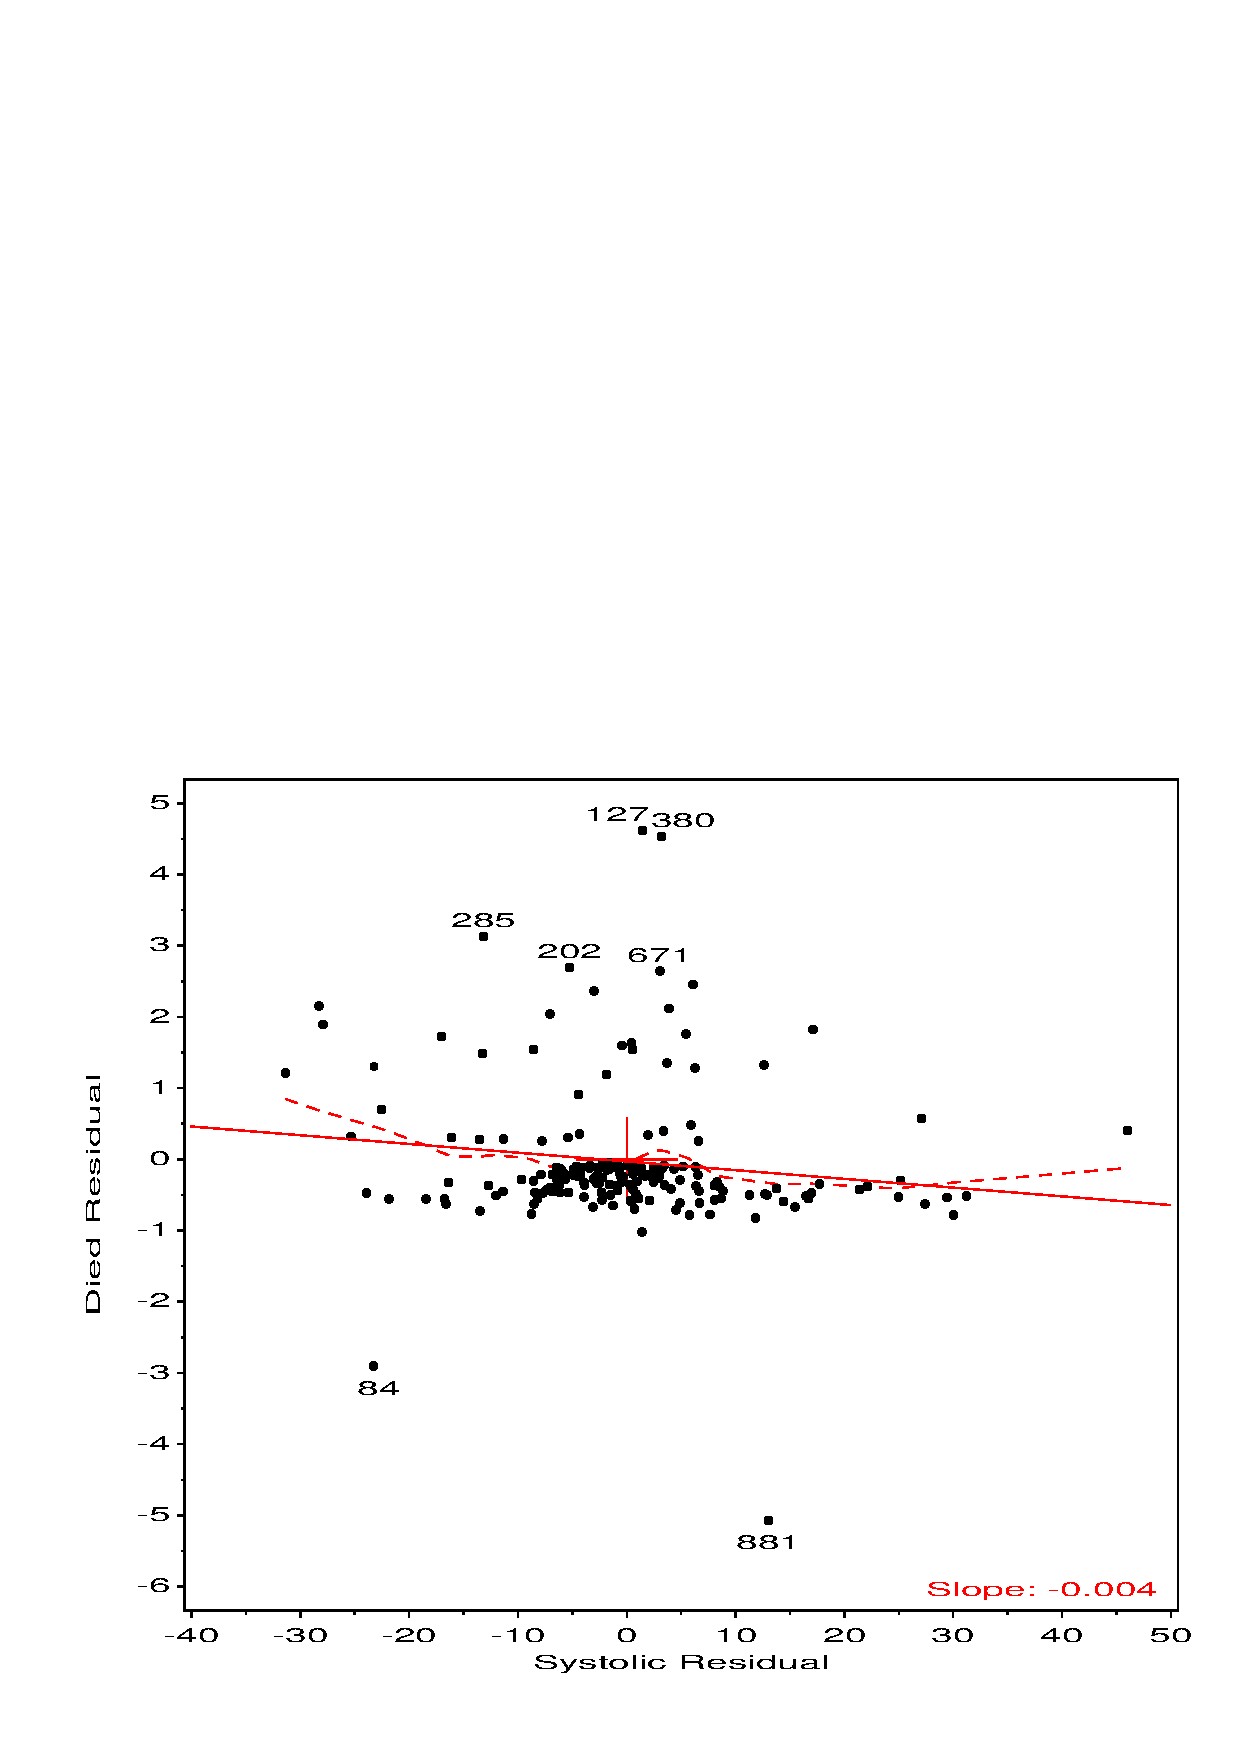
\includegraphics[scale=.6]{ch6/fig/icu61}
  \caption[ICU data: Added variable plot for Systolic blood pressure]{ICU data: Added variable plot for Systolic blood pressure.
 The solid line shows the weighted least squares regression of residuals
 on the Systolic residuals.  The broken curve is the lowess smooth.}%
  \label{fig:icu61}
\end{figure}

The added variable plot may also be used to determine if a regressor
should be included with an additional polynomial term.
For example we might check to see if Age${}^2$ should be included
in the model.  The statements below produce \figref{fig:icu62}.
\begin{listing}
data icu;
   set icu;
   age2 = .01 * (age-57.5)**2;

%addvar(data=icu, y=Died,  x=age admit cancer uncons, z=Age2,
   id=patient, smooth=0);
\end{listing}

%% one figure
\begin{figure}[htb]
  \centering
  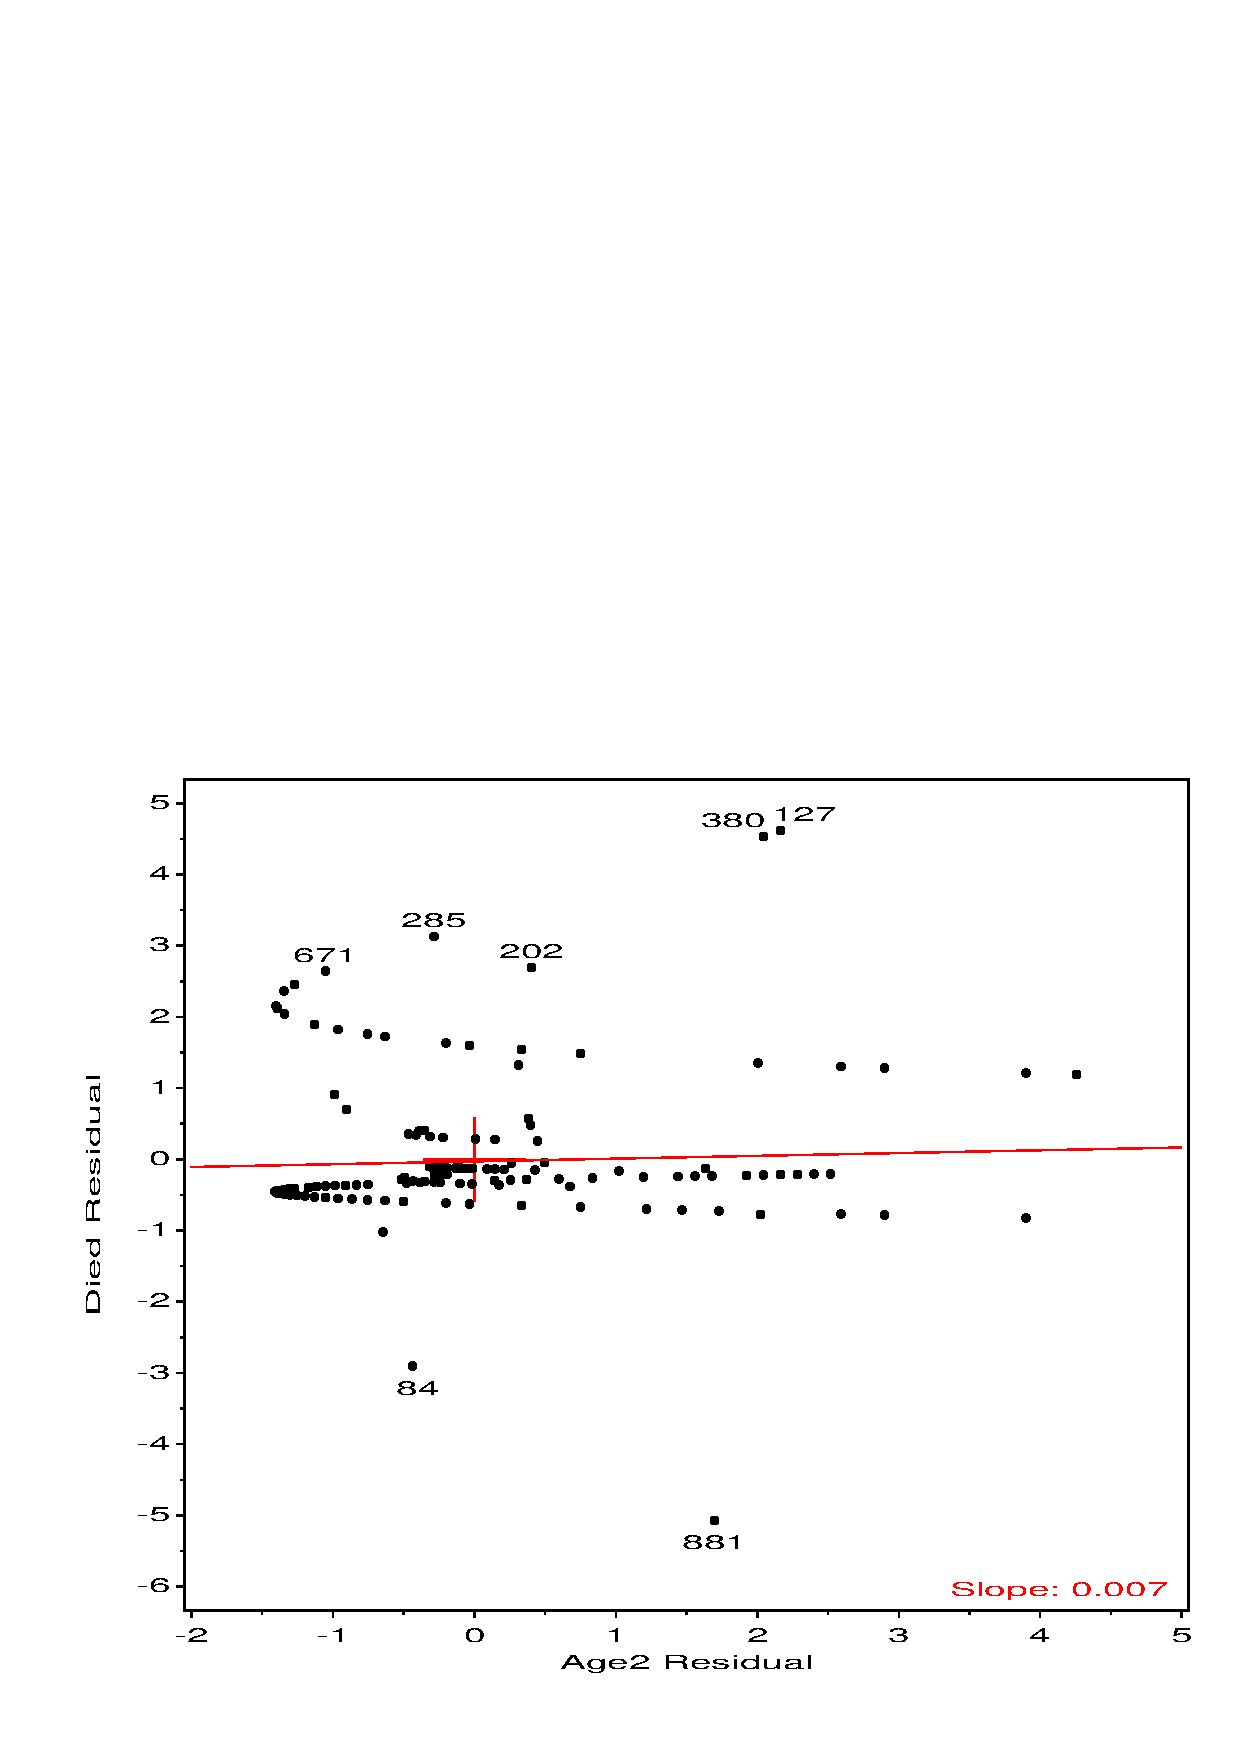
\includegraphics[scale=.6]{ch6/fig/icu62}
  \caption{ICU data: Added variable plot for Age${}^2$}%
  \label{fig:icu62}
\end{figure}
The slope of the line in \figref{fig:icu62} is approximately zero,
so we conclue that the squared term in Age is unnecessary.
\end{Example}

\subsubsection{Constructed variable plots}
While the partial residual plot is designed to detect a nonlinear relation
between the response and an explanatory variable,
it does not indicate the required transformation explicitly
and sometimes fails to diagnose nonlinearity
\citep{FienbergGong:84}.
The constructed variable plot, suggested for OLS regression
by \citet{Atkinson:81} and
\citet[\S 2.4.4]{CookWeisberg:82}, is specifically designed to
detect nonlinear dependence \emph{and} to suggest a power transformation
of the explanatory variable which would make the relation linear.
This plot was extended to generalized linear models by
\citet{WangP:87}.

Suppose that the variable $x_j$ is included in the model, and we are
contemplating replacing $x_j$  by a power $x_j^{(\lambda)}$ , defined by
the family \citep{BoxCox:64}
\begin{equation}\label{eq:boxcox}
x ^{(\lambda)} = \left\{
\begin{array}{cl}
\frac{x^\lambda - 1}{\lambda}, & \lambda \ne 0 \\
\log (x),  & \lambda = 0 \\
\end{array}
\right. \period
\end{equation}
To determine if a transformation is necessary, the constructed variable,
$z_j = b_j x_j \log x_j$ is calculated, where
$b_j$ is the estimated coefficient for $x_j$ in the original model.
Then the constructed variable plot is just an added variable plot for
$z_j$.

A linear trend, with a non-zero slope $\gamma$, in the constructed variable
plot indicates that a transformation of $x_j$ is necessary,
and the estimate of the power transformation in \eqref{eq:boxcox} is
$\hat{\lambda} = 1 + \gamma$, usually rounded to the nearest half-integer.
The absence of a linear trend means that $x_j$ is linear in the model.

